% Appendix B

\chapter{wxMaxima session code for producing picture \ref{fig:tax}} % Main appendix title

\label{Appendix_B} % For referencing this appendix elsewhere, use \ref{Appendix_B}

First, we solve the FOC. of the social planner's maximization problem. 


\noindent
%%%%%%%%%%%%%%%
%%% INPUT:
\begin{minipage}[t]{8ex}\color{red}\bf
(\% i1) 
\end{minipage}
\begin{minipage}[t]{\textwidth}\color{blue}
solve([-q[1]+5-q[1]-q[2]=s[1], -q[2]+5-q[1]-q[2]=s[2]], [q[1],q[2]] );
\end{minipage}
%%% OUTPUT:
\[\displaystyle
\tag{\% o1} 
[[{q_1}=-\frac{-{s_2}+2 {s_1}-5}{3},{q_2}=\frac{-2 {s_2}+{s_1}+5}{3}]]\mbox{}
\]
%%%%%%%%%%%%%%%
Price p: 


\noindent
%%%%%%%%%%%%%%%
%%% INPUT:
\begin{minipage}[t]{8ex}\color{red}\bf
(\% i2)
\end{minipage}
\begin{minipage}[t]{\textwidth}\color{blue}
p: ratsimp(5-(-(-s[2]+2*s[1]-5)/3+(-2*s[2]+s[1]+5)/3));
\end{minipage}
%%% OUTPUT:
\[\displaystyle
\tag{p}
\frac{{s_2}+{s_1}+5}{3}\mbox{}
\]
%%%%%%%%%%%%%%%
Second, calculate agent 1 's profit f(x,s\_1) given the share 2/3,1/3, and s\_2=1. 


\noindent
%%%%%%%%%%%%%%%
%%% INPUT:
\begin{minipage}[t]{8ex}\color{red}\bf
(\% i3)
\end{minipage}
\begin{minipage}[t]{\textwidth}\color{blue}
 ratsimp(1/3 * (-2+x+5)/3 *((1+x+5)/3 - 1)  + 2/3 * (-(-1+2*x-5)/3 *((1+x+5)/3 -s[1])));
\end{minipage}
%%% OUTPUT:
\[\displaystyle
\tag{\% o3} 
-\frac{{{x}^{2}}+\left( 2-4 {s_1}\right)  x+12 {s_1}-27}{9}\mbox{}
\]
%%%%%%%%%%%%%%%


\noindent
%%%%%%%%%%%%%%%
%%% INPUT:
\begin{minipage}[t]{8ex}\color{red}\bf
(\% i4)
\end{minipage}
\begin{minipage}[t]{\textwidth}\color{blue}
f(x,s) := -(x\^{}2+(2-4*s)*x+12*s-27)/9;
\end{minipage}
%%% OUTPUT:
\[\displaystyle
\tag{\% o4} 
\operatorname{f}\left( x,s\right) :=\frac{-\left( {{x}^{2}}+\left( 2-4 s\right)  x+12 s-27\right) }{9}\mbox{}
\]
%%%%%%%%%%%%%%%
Third, calculate the partial derivative of f(x,s) to x at s=x, and then from the differential equation \ensuremath{\partial}t(x)/\ensuremath{\partial}x=\ensuremath{\partial}f(x,s)/\ensuremath{\partial}x hold whens=x, we derive a t(x). 


\noindent
%%%%%%%%%%%%%%%
%%% INPUT:
\begin{minipage}[t]{8ex}\color{red}\bf
(\% i5)
\end{minipage}
\begin{minipage}[t]{\textwidth}\color{blue}
diff(f(x,s),x);
\end{minipage}
%%% OUTPUT:
\[\displaystyle
\tag{\% o5} 
\frac{-2 x+4 s-2}{9}\mbox{}
\]
%%%%%%%%%%%%%%%


\noindent
%%%%%%%%%%%%%%%
%%% INPUT:
\begin{minipage}[t]{8ex}\color{red}\bf
(\% i6)
\end{minipage}
\begin{minipage}[t]{\textwidth}\color{blue}
partial: (2*x-2)/9;
\end{minipage}
%%% OUTPUT:
\[\displaystyle
\tag{partial}
\frac{2 x-2}{9}\mbox{}
\]
%%%%%%%%%%%%%%%


\noindent
%%%%%%%%%%%%%%%
%%% INPUT:
\begin{minipage}[t]{8ex}\color{red}\bf
(\% i7)
\end{minipage}
\begin{minipage}[t]{\textwidth}\color{blue}
desolve('diff(t(x),x) =(2*x-2)/9, t(x));
\end{minipage}
%%% OUTPUT:
\[\displaystyle
\tag{\% o7} 
\operatorname{t}(x)=\frac{{{x}^{2}}}{9}-\frac{2 x}{9}+\operatorname{t}(0)\mbox{}
\]
%%%%%%%%%%%%%%%
We find from the following that all f(x,s)s go through (3,4/3), and let t(x) goes through it too, we get a tax(x). 


\noindent
%%%%%%%%%%%%%%%
%%% INPUT:
\begin{minipage}[t]{8ex}\color{red}\bf
(\% i8)
\end{minipage}
\begin{minipage}[t]{\textwidth}\color{blue}
ratsimp(f(3,s));
\end{minipage}
%%% OUTPUT:
\[\displaystyle
\tag{\% o8} 
\frac{4}{3}\mbox{}
\]
%%%%%%%%%%%%%%%


\noindent
%%%%%%%%%%%%%%%
%%% INPUT:
\begin{minipage}[t]{8ex}\color{red}\bf
(\% i9)
\end{minipage}
\begin{minipage}[t]{\textwidth}\color{blue}
tax(x) := x\^{}2/9-(2*x)/9+1;
\end{minipage}
%%% OUTPUT:
\[\displaystyle
\tag{\% o9} 
\operatorname{tax}(x):=\frac{{{x}^{2}}}{9}-\frac{2 x}{9}+1\mbox{}
\]
%%%%%%%%%%%%%%%


\noindent
%%%%%%%%%%%%%%%
%%% INPUT:
\begin{minipage}[t]{8ex}\color{red}\bf
(\% i10)
\end{minipage}
\begin{minipage}[t]{\textwidth}\color{blue}
tax(3);
\end{minipage}
%%% OUTPUT:
\[\displaystyle
\tag{\% o10} 
\frac{4}{3}\mbox{}
\]
%%%%%%%%%%%%%%%
Now we can draw the picture. 


\noindent
%%%%%%%%%%%%%%%
%%% INPUT:
\begin{minipage}[t]{8ex}\color{red}\bf
(\% i11)
\end{minipage}
\begin{minipage}[t]{\textwidth}\color{blue}
wxplot2d([f(x,0.1),f(x,1.0),f(x,1.2),f(x,1.8), f(x,3), tax(x)], [x, 0,6],[legend, "f(x,0.1)","f(x,1.0)","f(x,1.2)","f(x,1.8)", "f(x,3)", "tax(x)"]);


\end{minipage}

%\begin{figure}
%\centering
%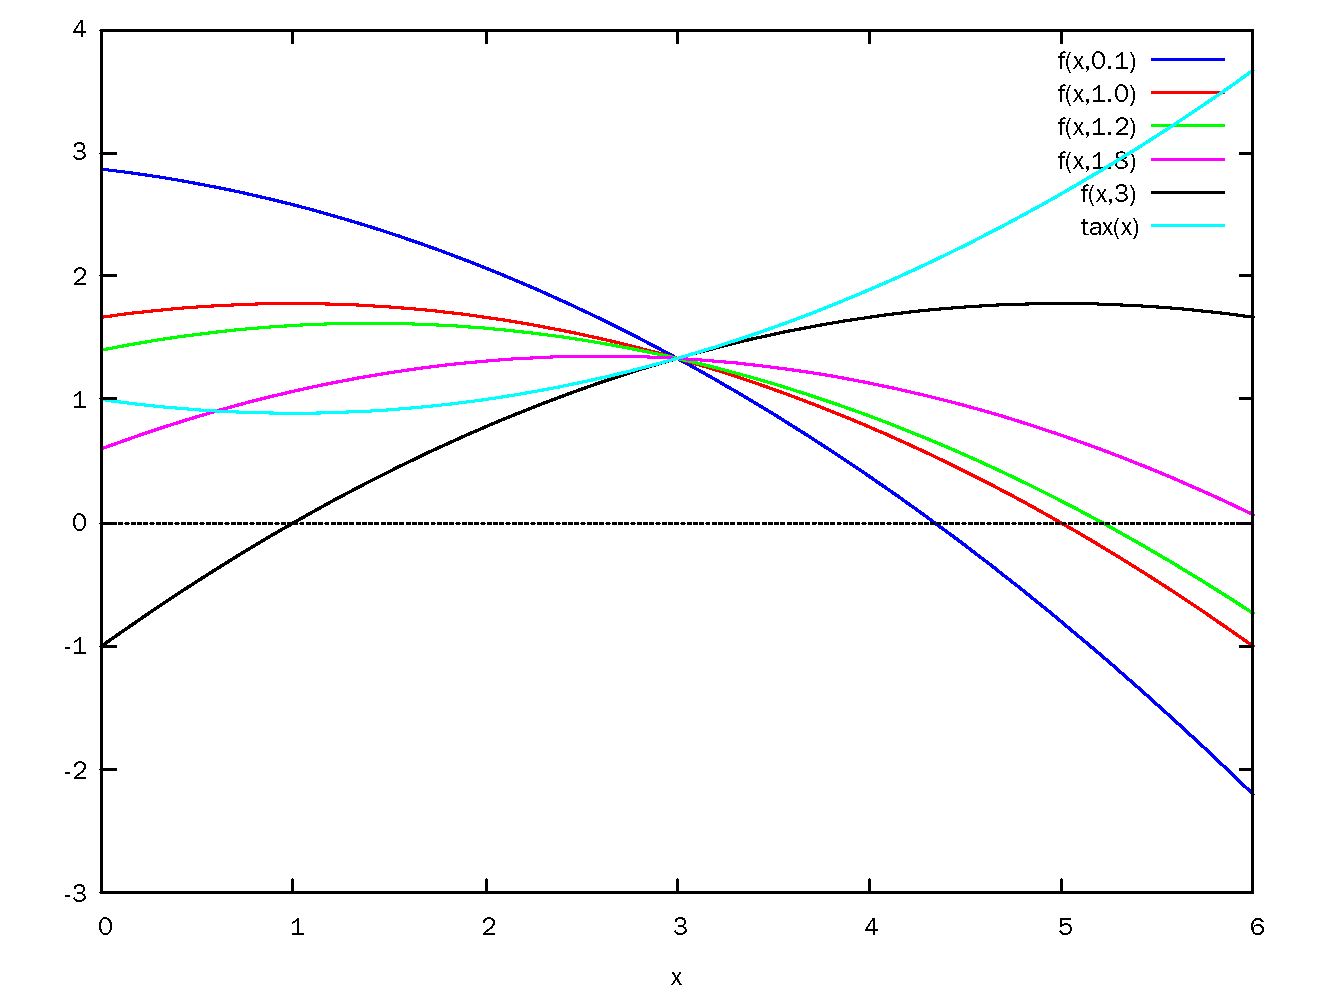
\includegraphics[width = 11cm]{tax.pdf}
%\caption{tax scheme $tax(x)$ etc.} \label{fig:transfer}
%\end{figure}

%%% OUTPUT:
%\[\displaystyle
%\tag{\% t11} 
%\includegraphics[width=.95\linewidth,height=.80\textheight,keepaspectratio]{tax_img/tax_1}\mbox{}
%\]
%%%%%%%%%%%%%%%



